\chapter{Grid HTM}
\label{sec:grid_htm}
This chapter presents Grid HTM, which is the product of answering the thesis question and is the main contribution of this thesis. The source code of Grid HTM can be found on Github\cite{master_thesis_github}.
\section{Introduction}
\par
This thesis explores a new type of architecture, named Grid HTM, for anomaly detection in videos using \gls*{htm}, and proposes to use segmentation techniques to simplify the data into an SDR-friendly format. These segmentation techniques could be anything from simple binary thresholding to deep learning instance segmentation. Even keypoint detectors such as ORB~\cite{orb_detector} could in theory be applied. When explaining Grid HTM, the examples will be taken from deep learning instance segmentation of cars on a video from the VIRAT~\cite{VIRAT} dataset. An example segmentation is shown in \autoref{fig:example_segmentation}.
\begin{figure}[H]
    \centering
    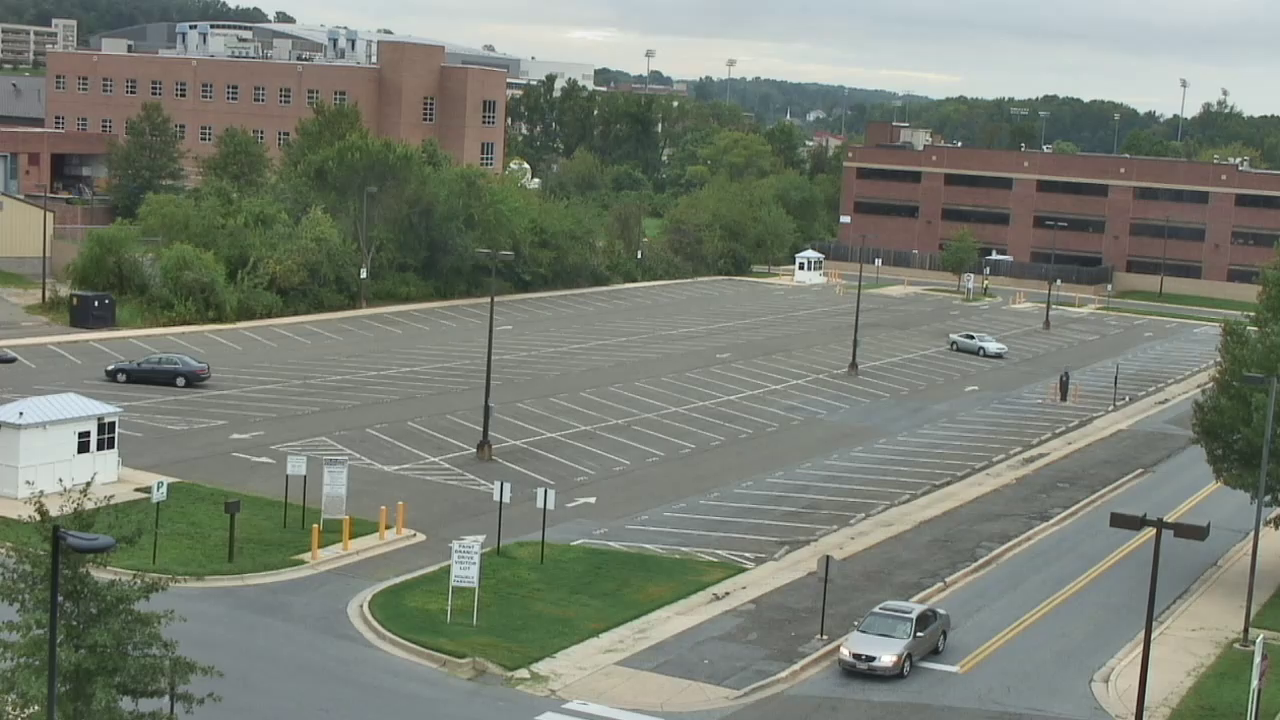
\includegraphics[width=.45\textwidth]{resources/methodology/original.png}
    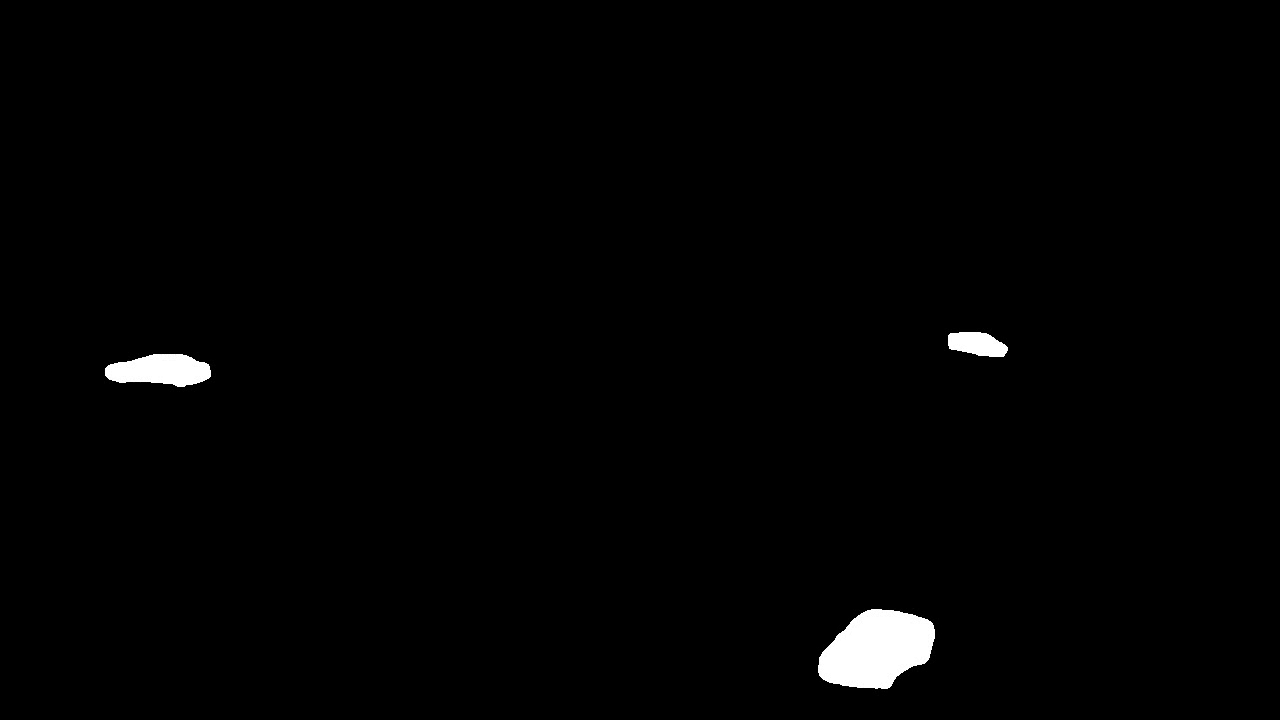
\includegraphics[width=.45\textwidth]{resources/methodology/car_segmentation.png}
    \caption[Segmentation Result of Cars]{Segmentation result of cars, which is suited to be used as an SDR. Original frame taken from VIRAT~\cite{VIRAT}.}
    \label{fig:example_segmentation}
\end{figure}
The idea is that the \gls*{sp} will learn to find an optimal general representation of cars. How general this representation is can be configured using the various parameters, but ideally they should be set so that different cars will be represented similarly while trucks and motorcycles will be represented differently. An example representation by the SP is shown in \autoref{fig:car_segmentation_sp}.
\begin{figure}[H]
    \centering
    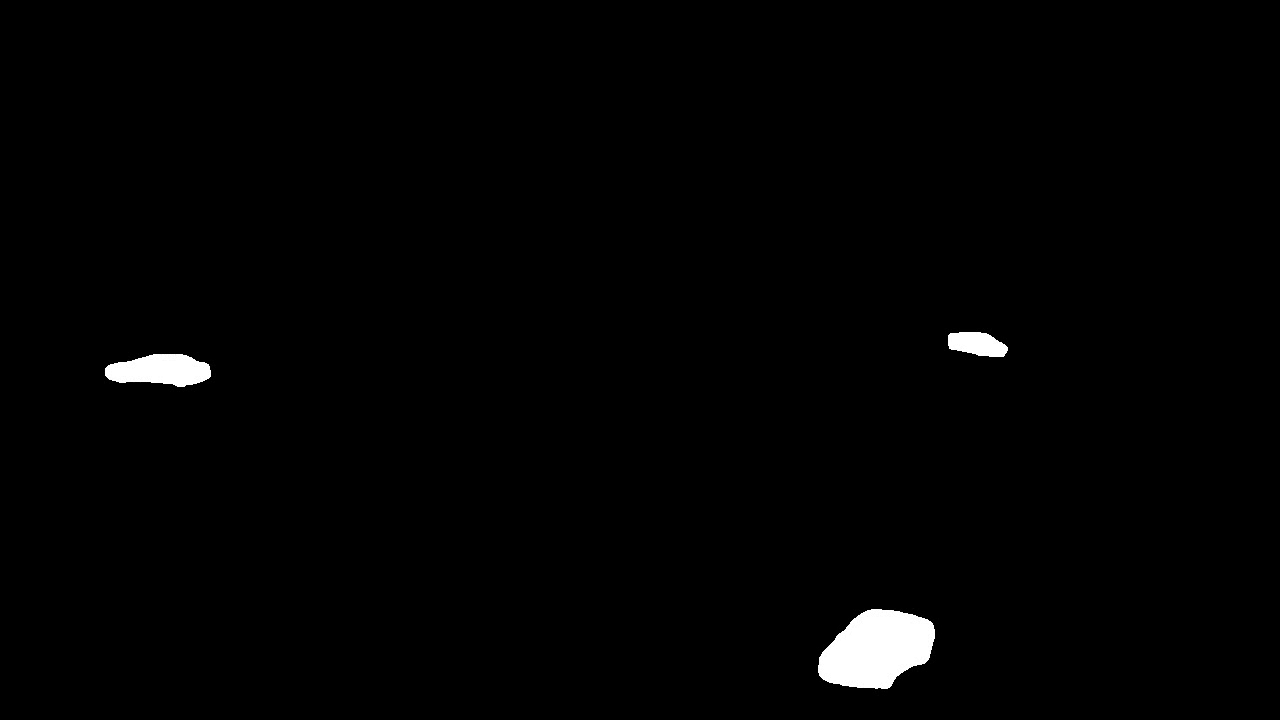
\includegraphics[width=.48\textwidth]{resources/methodology/car_segmentation.png}
    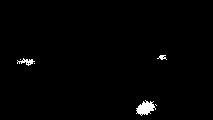
\includegraphics[width=.48\textwidth]{resources/methodology/car_segmentation_sp.png}
    \caption[SDR and SP Representation]{The SDR (left) and its corresponding \gls*{sp} representation (right). Note that the \gls*{sp} is untrained.}
    \label{fig:car_segmentation_sp}
\end{figure}
\par
The task of the \gls*{tm} will then be to learn the common patterns that the cars exhibit, their speed, shape, and positioning will be taken into account. Finally, the learning will be set so that new patterns are learned quickly, but forgotten slowly. This will allow the model to quickly learn the norm, even if there is little activity, while still reacting to anomalies. This requires that the input is stationary, in our example this means that the camera is not moving.
\par
It is possible to split different segmentation classes into their respective SDRs. This will give the SP and the TM the ability to learn different things for each of the classes. For instance, if there are two classes "person" and "car", then the TM will learn that it is normal for objects belonging to "person" to be on the sidewalk, while objects belonging to "car" will be marked as anomalous when on the sidewalk.
\par
Ideally, the architecture will have a calibration period spanning several days or weeks, during which the architecture is not performing any anomaly detection, but is just learning the patterns.
\section{Improvements}
As it currently stands, the current architecture is nearly identical to the one used by \textcite{MotionAnomalyDetection}, which was shown to not be particularly effective, therefore multiple improvements are introduced to increase effectiveness.
\subsection{Invariance}
One issue that becomes evident is the lack of invariance, due to the \gls*{tm} learning the global patterns. Using the example, it learns that it is normal for cars to drive along the road but only in the context of there being cars parked in the parking lot. It is instead desired that the \gls*{tm} learns that it is normal for cars to drive along the road, regardless of whether there are cars in the parking lot.
\par
This thesis proposes a solution based on dividing the encoder output into a grid (see \autoref{fig:grid}), and have a separate \gls*{sp} and \gls*{tm} for each cell in the grid. The anomaly scores of all the cells are then aggregated into a single anomaly score using an aggregation function.
\begin{figure}[H]
    \centering
    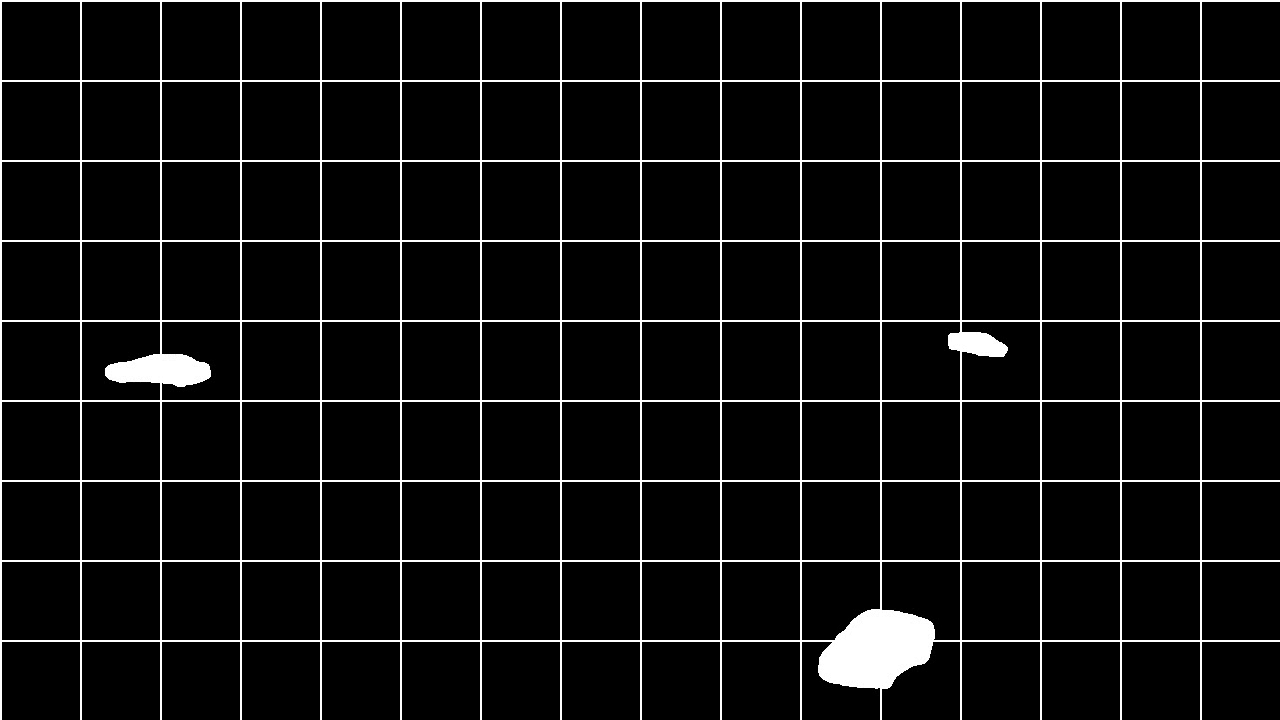
\includegraphics[width=\textwidth]{resources/methodology/car_segmentation_grid.png}
    \caption[Encoder Output Grid]{The encoder output divided into a grid.}
    \label{fig:grid}
\end{figure}
\subsubsection{Aggregation Function}
Selecting the correct aggregation function is important because it affects the final anomaly output. For instance, it might be tempting to use the mean of all the anomaly scores as the aggregation function:
\begin{align*}
    X         & :\{x \in \mathbb{R} : x \geq 0\}     \\
    \\
    anomScore & =\dfrac{\sum\limits_{x \in X}x}{|X|}
\end{align*}
However, this leads to problems with normalization, meaning that an overall anomaly score of 1 is hard to achieve due to many cells having a zero anomaly score. In fact, it becomes unclear what a high anomaly score is anymore. Using the mean also means that anomalies that take up a lot of space will be weighted more than anomalies that take up a little space, which might not be desirable.
\par
To solve the aforementioned problem and if the data has little noise, a potential aggregation function could be the non-zero mean:
\begin{align*}
    X         & :\{x \in \mathbb{R} : x > 0\} \\
    \\
    anomScore & =
    \begin{cases}
        \dfrac{\sum\limits_{x \in X}x}{|X|} & \text{if } |X| > 0 \\
        \\
        \hfil 0                             & \text{otherwise}
    \end{cases}
\end{align*}
Meaning that only the cells with a non-zero anomaly score, denoted $X$, will be contributing to the overall anomaly score which helps solve the aforementioned normalization and weighting problem. On the other hand, this will perform poorly when the architecture is exposed to noisy data which could lead to there always being one or more cells with a high anomaly score.
\begin{figure}[H]
    \centering
    Noisy data
    \begin{subfigure}[t]{0.5\textwidth}
        \centering
        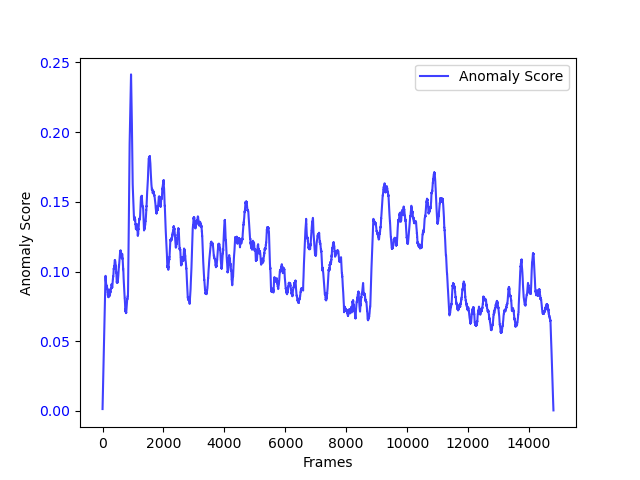
\includegraphics[width=\textwidth]{resources/methodology/aggr_noisy_mean.png}
        \caption{Mean.}
    \end{subfigure}%
    \begin{subfigure}[t]{0.5\textwidth}
        \centering
        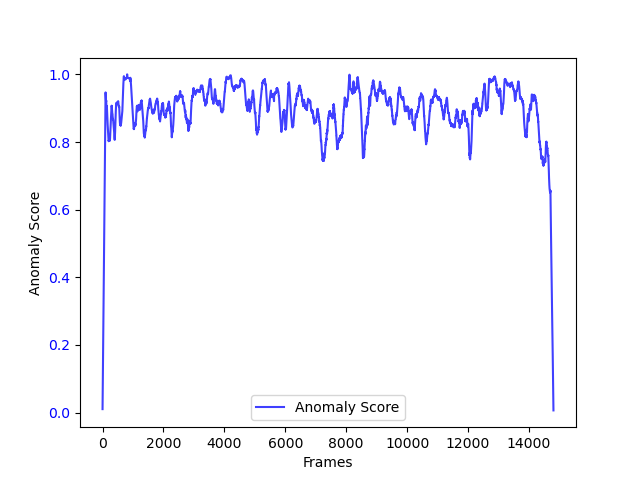
\includegraphics[width=\textwidth]{resources/methodology/aggr_noisy_nzmean.png}
        \caption{Non-zero mean.}
    \end{subfigure}
    \caption[Aggregation Functions on Noise Data]{How the two aggregation functions perform on the same noisy data.}
    \label{fig:aggr_noisy}
\end{figure}
\begin{figure}[H]
    \centering
    Clean data
    \begin{subfigure}[t]{0.5\textwidth}
        \centering
        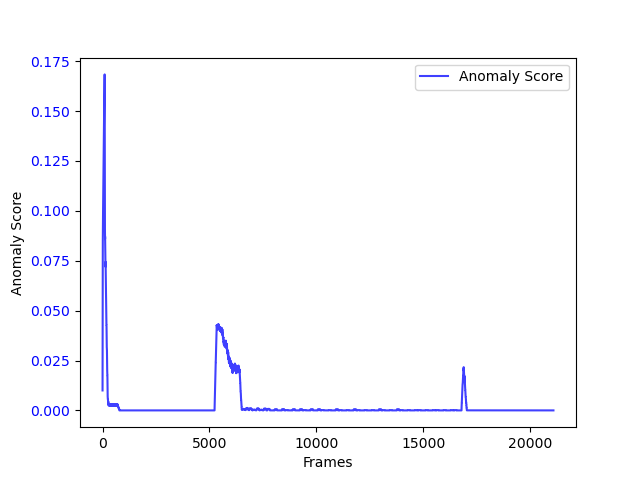
\includegraphics[width=\textwidth]{resources/methodology/aggr_clean_mean.png}
        \caption{Mean.}

    \end{subfigure}%
    \begin{subfigure}[t]{0.5\textwidth}
        \centering
        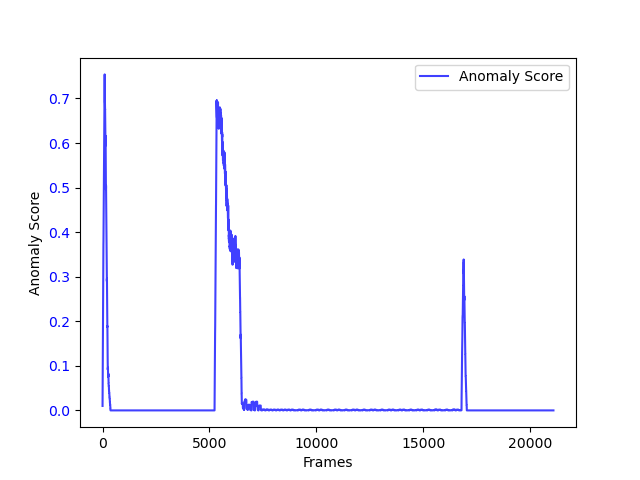
\includegraphics[width=\textwidth]{resources/methodology/aggr_clean_nzmean.png}
        \caption{Non-zero mean.}
    \end{subfigure}
    \caption[Aggregation Functions on Clean Data]{How the two aggregation functions perform on the same clean data.}
    \label{fig:aggr_clean}
\end{figure}
\autoref{fig:aggr_noisy} illustrates the effect of an aggregation function for noisy data, where the non-zero mean is rendered useless due to the noise. On the other hand, \autoref{fig:aggr_clean} shows how the non-zero mean gives a clearer anomaly score when the data is clean. Especially regarding how, unlike the mean, the non-zero mean has a clearly defined range between 0 and 1.
\subsection{Explainability}
Having the encoder output divided into a grid has the added benefit of introducing explainability into the model. By using Grid \gls*{htm} it is now possible to find out where in the input an anomaly has occurred by simply observing which cell has a high anomaly score.
\par
It is also possible to estimate the number of predictions for each cell which can be used as a measure of certainty, where fewer predictions means higher certainty. Making it possible to measure certainty per cell creates a new source of information which can be used for explainability or robustness purposes.
\par
These two properties show that GridHTM offers vastly more explainability than current state-of-the-art deep learning models for anomaly detection, which could make it an attractive approach.
\subsection{Flexibility and Performance}
In addition, it is also possible to configure the \gls*{sp} and the \gls*{tm} in each cell independently, giving the architecture increased flexibility. It is also possible to use a non-uniform grid, meaning that some cells can have different sizes. Last but not least, dividing the frame into smaller cells makes it possible to run each cell in parallel for increased performance.
\subsection{Reviewing Encoder Rules}
That being said, a potential problem with the grid approach is that the rules for creating a good encoder, mentioned in \autoref{sec:encoders}, may not be respected and therefore should be reviewed:
\begin{itemize}
    \item \textbf{Semantically similar data should result in SDRs with overlapping active bits}. In this example, a car at one position will produce an SDR with a high amount of overlapping bits as another car at a similar position in the input image.
    \item \textbf{The same input should always produce the same SDR}. The segmentation model produces a deterministic output given the same input.
    \item \textbf{The output must have the same dimensionality (total number of bits) for all inputs}. The segmentation model output has a fixed dimensionality.
    \item \textbf{The output should have similar sparsity (similar amount of one-bits) for all inputs and have enough one-bits to handle noise and subsampling}. The segmentation model does not respect this. An example is that there can be no cars (zero active bits), one car ($n$ active bits), or two cars ($2n$ active bits), and that this will fluctuate over time.
\end{itemize}
The solution for the last rule is two-fold, and  consists of imposing a soft upper bound and a hard lower bound for the number of active pixels within a cell. The purpose is to lower the variation of number of active pixels, while also containing enough semantic information for the \gls*{htm} to work:
\begin{itemize}
    \item Pick a cell size so that the distribution of number of active pixels is as tight as possible, while containing enough semantic information and also being small enough so that the desired invariance is achieved. The cell size acts as a soft upper bound for the possible number of active pixels.
    \item Create a pattern representing emptiness, where the number of active bits is similar to what can be expected on average when there are cars inside a cell. This acts as a hard lower bound for the number of active pixels.
\end{itemize}
There could be situations where a few pixels are active within a cell, which could happen when a car has just entered a cell, but this is fine as long as it does not affect the distribution too much. If it does affect the distribution, which can be the case with noisy data, then an improvement would be to add a minimum sparsity requirement before a cell is considered not empty, e.g. less than 5 active pixels means that the cell is empty.  In the following example, the number of active pixels within a cell centered in the video was used to build the distributions seen in \autoref{fig:num_active_pixels_dist}:
\begin{figure}[H]
    \centering
    \begin{subfigure}[t]{0.49\textwidth}
        \centering
        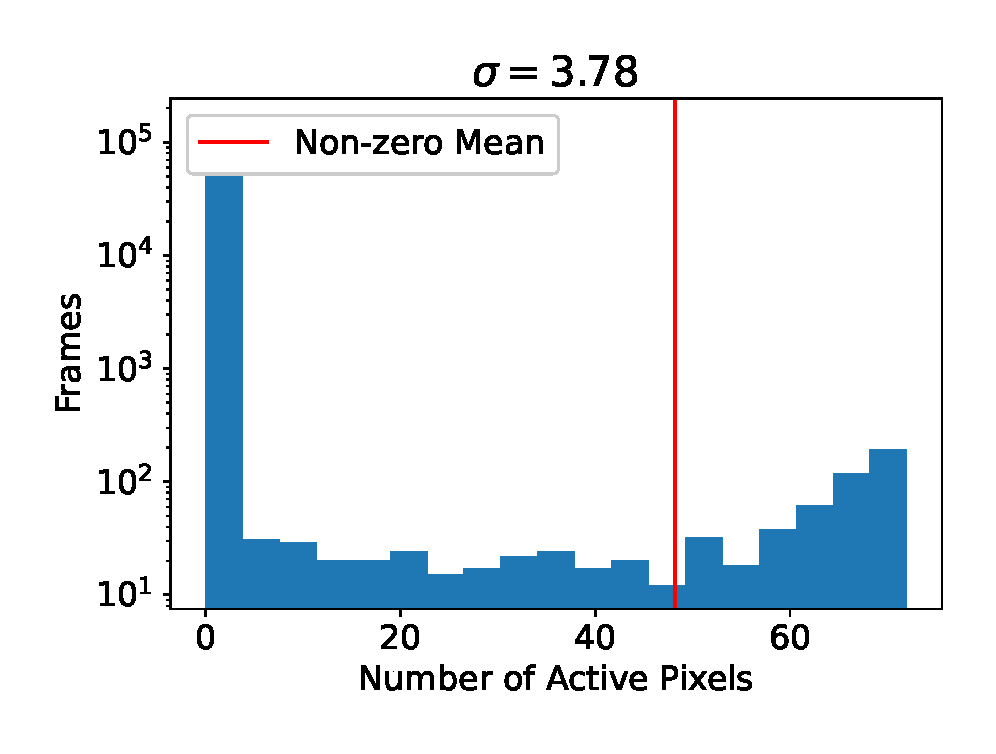
\includegraphics[width=\textwidth]{resources/methodology/active_pixels_dist.eps}
        \caption{Without empty pattern.}
    \end{subfigure}%
    \begin{subfigure}[t]{0.49\textwidth}
        \centering
        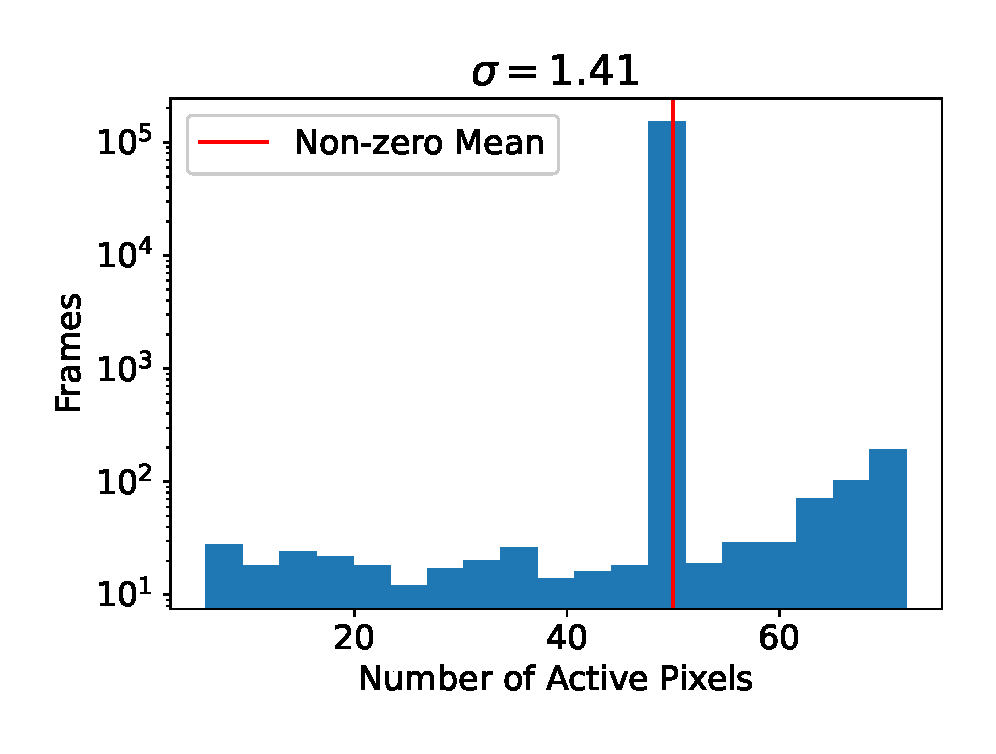
\includegraphics[width=\textwidth]{resources/methodology/active_pixels_dist2.eps}
        \caption{With empty pattern and a minimum sparsity requirement of $5$.}
    \end{subfigure}
    \caption[Distribution of Active Pixels]{Distribution of number of active pixels within a cell of size $12\times 12$.}
    \label{fig:num_active_pixels_dist}
\end{figure}


With a carefully selected empty pattern sparsity, \textbf{the standard deviation of active pixels was lowered from $\mathbf{3.78}$ to $\mathbf{1.41}$}. It is possible to automate this process by developing an algorithm which finds the optimal cell size and empty pattern sparsity which causes the least variation of number of active pixels per cell. This algorithm would run as a part of the calibration process.\par
The visual output resulting from these changes, which is an equally important output as the aggregated anomaly score, can be seen in \autoref{fig:gridhtm_output}.
\begin{figure}[H]
    \centering
    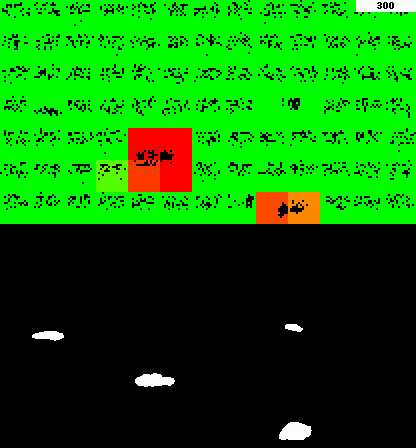
\includegraphics[width=0.7\textwidth]{resources/methodology/htm_grid_output.png}
    \caption[Example Grid HTM Output]{Example Grid \gls*{htm} output and the corresponding input. The color represents the anomaly score for each of the cells, where red means high anomaly score and green means zero anomaly score. Two of the cars are marked as anomalous because they are moving, which is something the Grid \gls*{htm} has not seen before during its 300 frame long lifetime.}
    \label{fig:gridhtm_output}
\end{figure}
Since there are now cells that are observing an empty pattern for a lot of the time in sparse data, boosting is recommended to be turned off, otherwise the \gls*{sp} output for the empty cells would change back and forth in order to adjust the active duty cycle.
\subsection{Stabilizing Anomaly Output}
\label{sec:stabilizing_anomaly_output}
\begin{figure}[H]
    \centering
    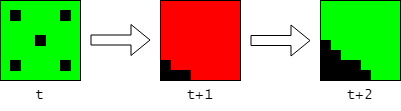
\includegraphics[width=0.7\textwidth]{resources/methodology/empty_to_notempty.png}
    \caption[Stabilizing Anomaly Output Visualization 1]{High anomaly score when an empty cell (represented with an empty pattern with a sparsity value of 5) changes to being not empty, as something enters the cell.}
    \label{fig:empty_to_notempty}
\end{figure}
Another issue with the grid based approach is when a car first comes into a cell. The \gls*{tm} in that cell has no way of knowing that a car is about to enter, since it does not see outside its own cell, and therefore the first frame that a car enters a cell will cause a high anomaly output. This is illustrated in \autoref{fig:empty_to_notempty} where it can be observed that this effect causes the anomaly output to needlessly fluctuate. The band-aid solution is to ignore the anomaly score for the frame during which the cell goes from being empty to being not empty, which is illustrated in \autoref{fig:empty_to_notempty_fixed}.
\begin{figure}[H]
    \centering
    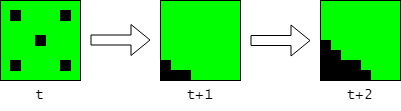
\includegraphics[width=0.7\textwidth]{resources/methodology/empty_to_notempty_fixed.png}
    \caption[Stabilizing Anomaly Output Visualization 2]{In this case, the anomaly score is ignored (set to 0) for the frame in which the cell changes state from empty to not empty.}
    \label{fig:empty_to_notempty_fixed}
\end{figure}
A more proper solution could be to allow the \gls*{tm} to grow synapses to the TMs in the neighboring cells, but this is not documented in any research papers and might also hinder invariance.
\subsection{Multistep Temporal Patterns}
\label{sec:multistep_temporal_patterns}
Since the \gls*{tm} can only grow segments to cells that were active in the previous timestep, as was mentioned in \autoref{sec:temporal_memory}, it will struggle to learn temporal patterns across multiple timesteps. This is especially evident in high framerate videos, where an object in motion has a similar representation at timestep $t$ and $t+1$, as an object standing still. \autoref{fig:high_fps} visualizes this phenomenon.
\begin{figure}[H]
    \centering
    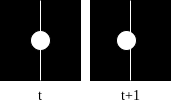
\includegraphics[width=0.3\textwidth]{resources/methodology/high_fps_moving.png}
    \unskip\ \vrule\
    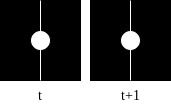
\includegraphics[width=0.3\textwidth]{resources/methodology/high_fps_still.png}
    \caption[Comparison of a Moving Object in a High Framerate Video]{Comparison of a moving object (left) and a still object (right) in a high framerate video. They are very similar and could actually end up being represented identically by the SP.}
    \label{fig:high_fps}
\end{figure}
This could cause situations where an object that is supposed to be moving, suddenly stands still, yet the \gls*{tm} will not mark it as an anomaly due to it being stuck in a contextual loop (see \autoref{fig:contextual_loop}). A contextual loop is when one of the predictions at $t$ becomes true at $t+1$, and then one of the predictions at $t+1$ is almost identical to the state at $t$, which becomes true if the object is not moving, causing the \gls*{tm} to enter the same state that it was in at $t$.
\begin{figure}[H]
    \centering
    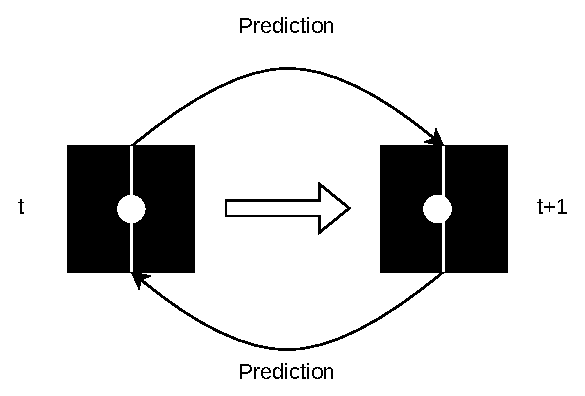
\includegraphics[width=0.7\textwidth]{resources/methodology/contextual_loop.eps}
    \caption[Contextual Loop Example]{Example of a contextual loop.}
    \label{fig:contextual_loop}
\end{figure}
A solution is to concatenate the past $n$ \gls*{sp} outputs as input into the TM, which is made possible by keeping a buffer of past \gls*{sp} outputs and shifting its contents out as new \gls*{sp} outputs are inserted (see \autoref{fig:mtp}). This follows the core idea behind encoding time in addition to the data, which makes time act as a contextual anchor. However, in this case there are no timestamps that are suitable to be used as contextual anchors, so as a replacement, the past observations are encoded instead. Parallels can be drawn to the Transformer model, where a positional encoding is required for it to learn order of sequences~\cite{transformer}.
\par
\begin{figure}[H]
    \centering
    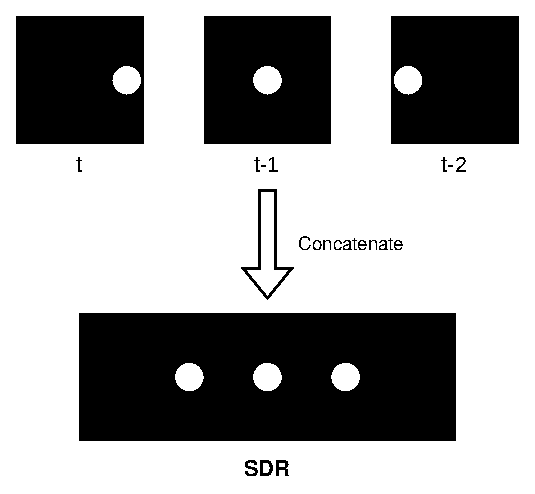
\includegraphics[width=0.45\textwidth]{resources/methodology/temporal_concatenation.eps}
    \unskip\ \vrule\
    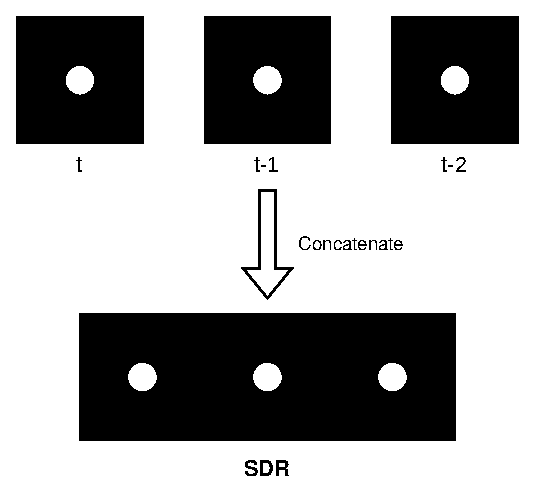
\includegraphics[width=0.45\textwidth]{resources/methodology/temporal_concatenation_still.eps}
    \caption[Multistep Temporal Pattern Example]{Example of concatenation with $n=3$ when an object is moving from left to right, compared to when an object is not in motion. It can be observed that the SDRs are vastly different.}
    \label{fig:mtp}
\end{figure}
Concatenating past observations together will force the \gls*{tm} input, for when an object is in motion and when an object is still, to be unique. High framerate videos can benefit the most from this, and the effect will be more pronounced for higher values of $n$. One could feed the past $n$ encoder outputs into the \gls*{sp} instead, but this will lead to a much higher computational requirement, as well as make both the \gls*{sp} and \gls*{tm} parameters to be dependent on $n$.

\par
A potential side effect of introducing temporal patterns, is that because the TM is now exposed to multiple frames at once, it will be more tolerant to temporal noise. An example of temporal noise is when an object disappears for a single frame due to falling below the classification threshold of the deep learning segmentation model encoder. The reason for the noise tolerance is that instead of the temporal noise making up the entire input for the TM, it now only makes up $\frac{1}{n}$ of the TM input.
\par
Adding support for multistep temporal patterns to the method used by \textcite{MotionAnomalyDetection}, which is mentioned in \autoref{sec:htm_perf}, could improve their results.
\section{Implementation}
Grid HTM was implemented in Python using the community fork of Numenta's HTM codebase~\cite{htm_community_fork}. The reason for using the community fork is that Numenta has stopped developing the original codebase, and that the community codebase is more optimized and has more features. There are other HTM implementations available~\cite{htm_community_cuda,htm_community_brainblocks}, but these were not considered due to their low popularity meaning that they have a higher chance of lacking features and containing bugs.
\section{Biological Plausibility}
One of the key principles of HTM theory is that it should be biologically plausible~\cite{BAMI}. Every development within HTM theory follows this principle, and it should therefore be expected that Grid HTM does so as well.
\par
Remembering that a single HTM model models a cortical column, as stated in \autoref{sec:htm_structure}, means that each cell in the grid can be considered an individual cortical column. The entire architecture can therefore be thought of as a simplified cortical region, as visualized in \autoref{fig:cortical_region}.
\section{Use Cases}
\begin{figure}[H]
    \centering
    \begin{subfigure}{0.49\linewidth}
        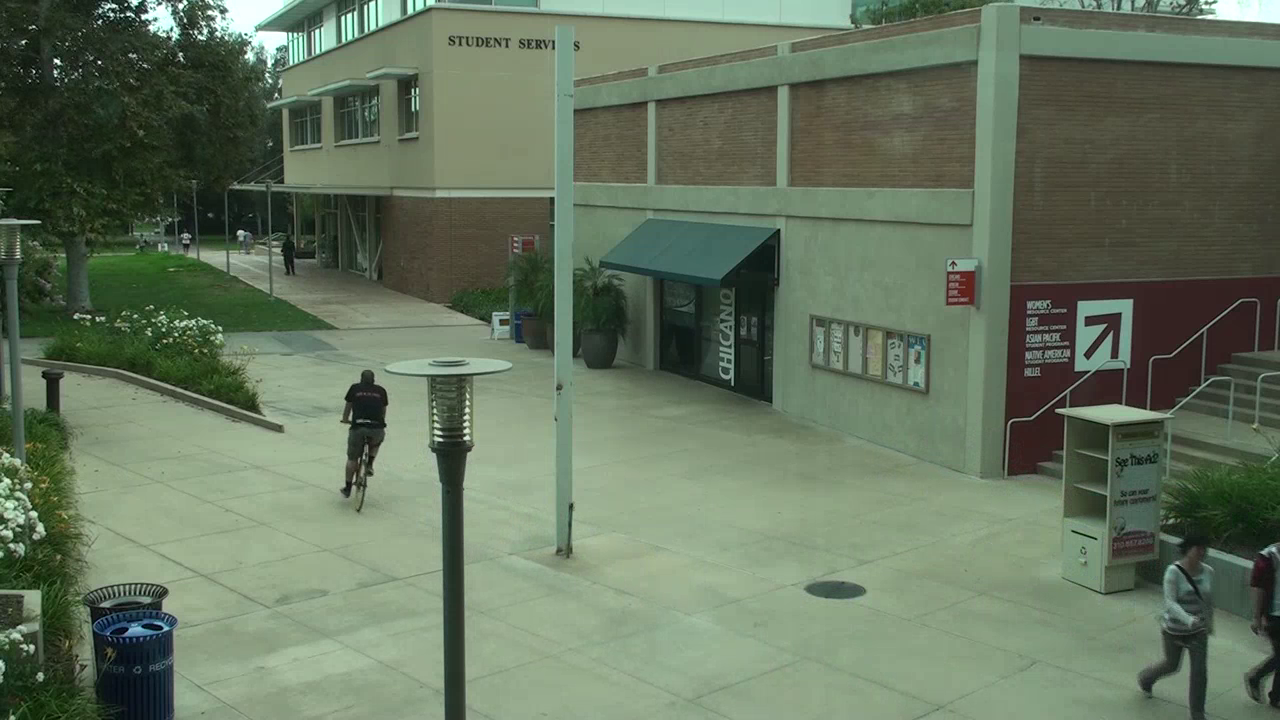
\includegraphics[width=\linewidth]{resources/methodology/surveillance_example1.png}
    \end{subfigure}
    \begin{subfigure}{0.49\linewidth}
        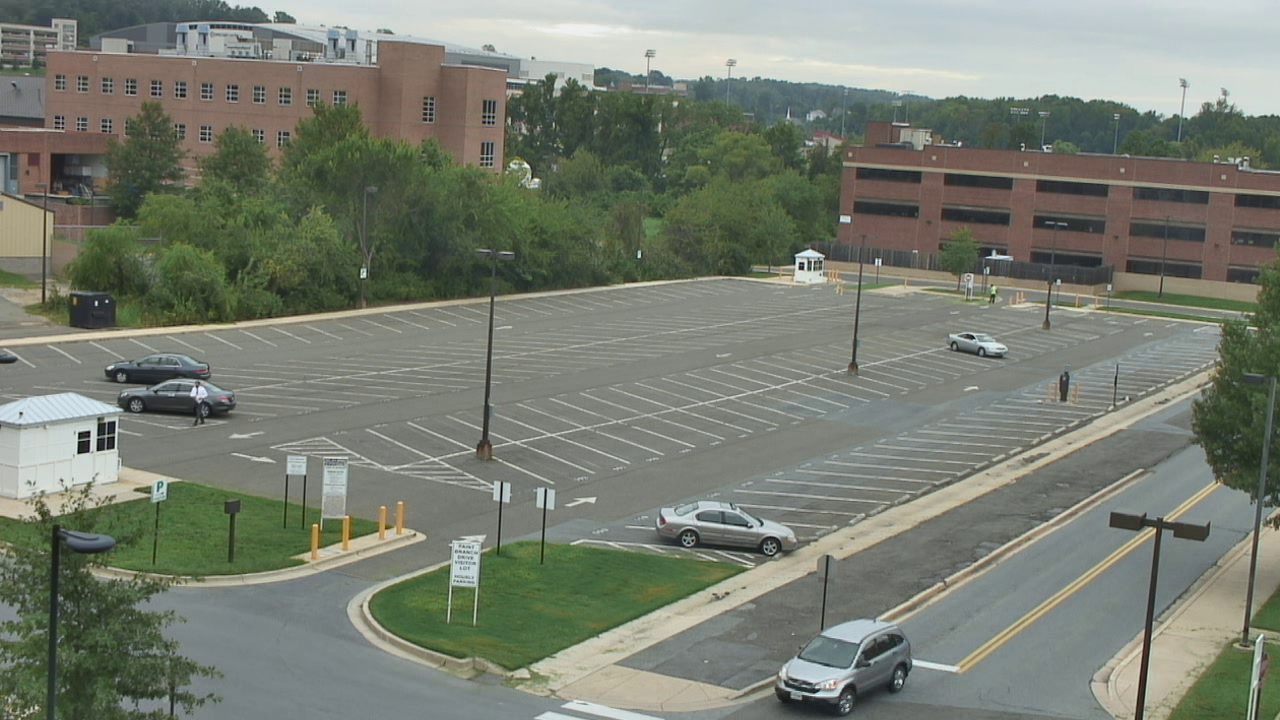
\includegraphics[width=\linewidth]{resources/methodology/surveillance_example2.png}
    \end{subfigure}
    \begin{subfigure}{0.49\linewidth}
        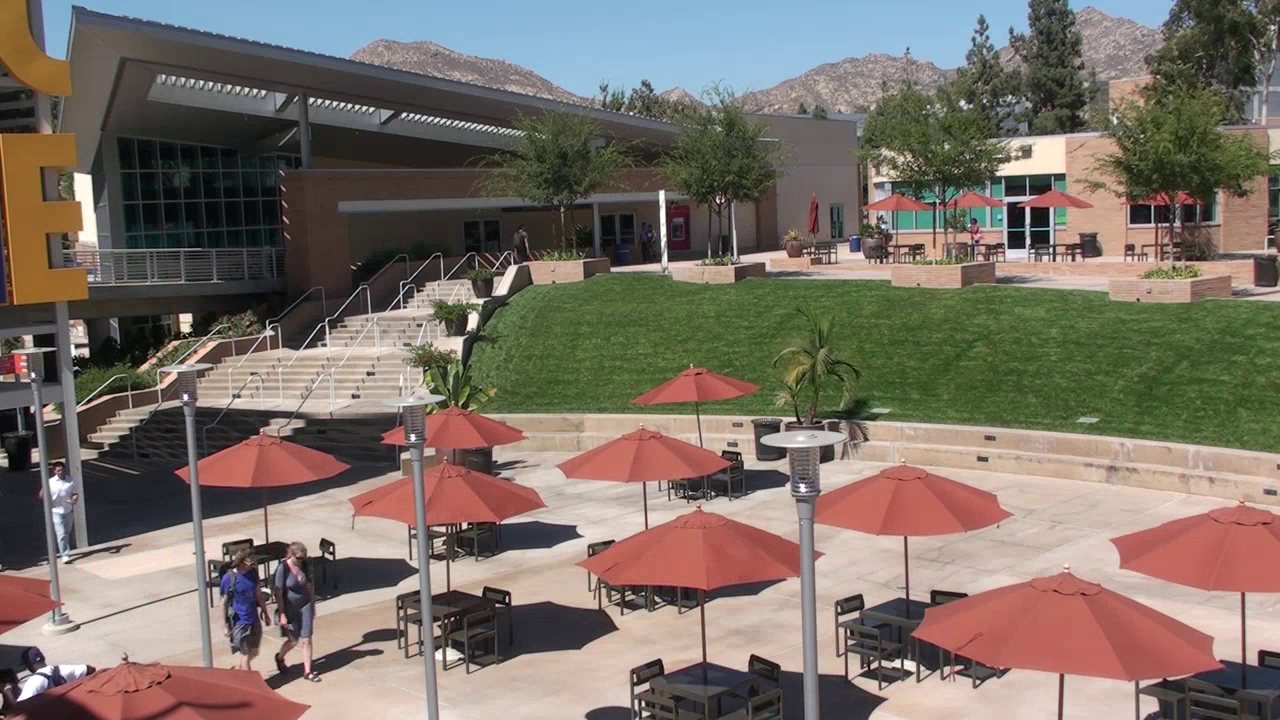
\includegraphics[width=\linewidth]{resources/methodology/surveillance_example3.png}
    \end{subfigure}
    \begin{subfigure}{0.49\linewidth}
        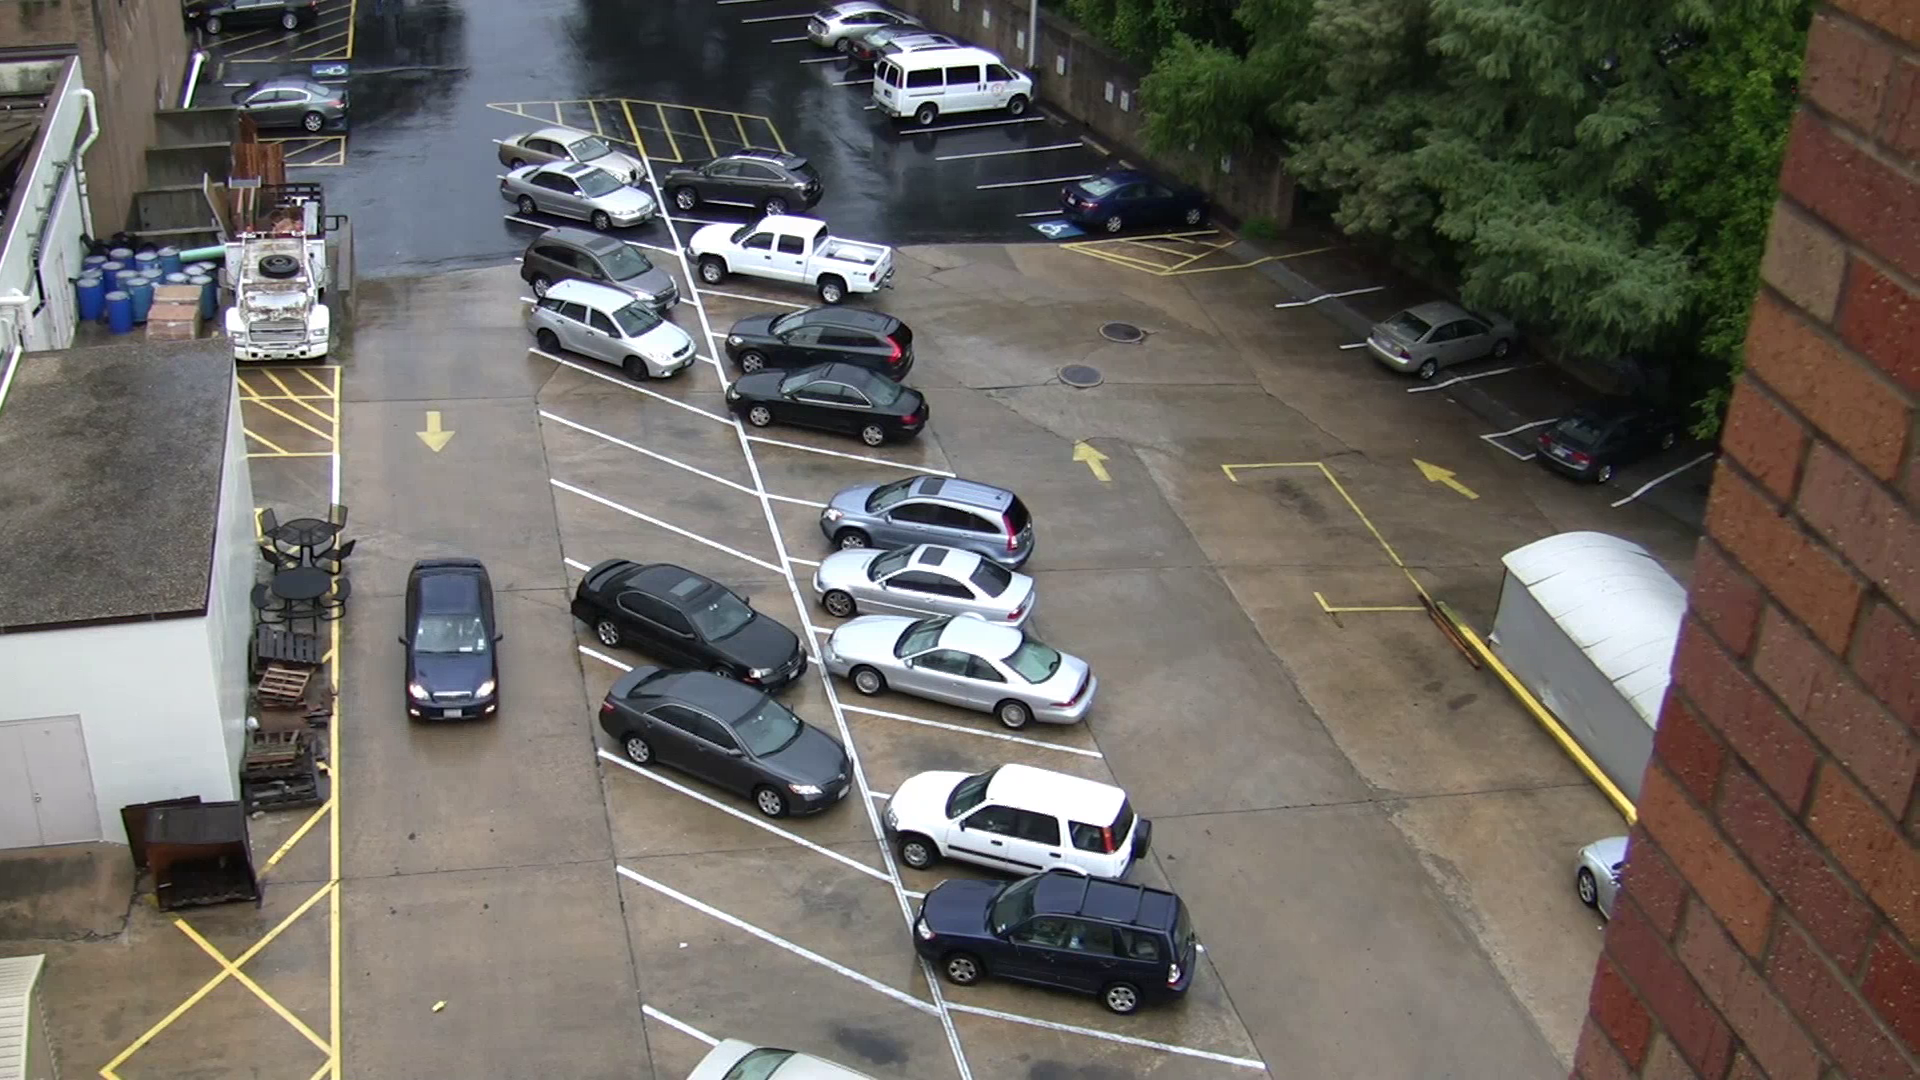
\includegraphics[width=\linewidth]{resources/methodology/surveillance_example4.png}
    \end{subfigure}
    \caption[Grid HTM Environments]{Examples of environments that Grid HTM could help monitor. Images taken from the VIRAT~\cite{VIRAT} dataset.}
    \label{fig:virat_examples}
\end{figure}
The most intuitive use case is to use Grid \gls*{htm} for semi-active surveillance, where personnel only have to look at segments containing anomalies, leading to drastically increased efficiency.
\par
One example is making it possible to have an entire city, with environments such as in \autoref{fig:virat_examples}, be monitored by a few people. This is made possible by making it so that people only have to look at segments that the Grid \gls*{htm} has found anomalous, which is what drastically lowers the manpower requirement for active monitoring of the entire city.
\par
Grid HTM could also be used to help automate labeling of anomaly datasets for deep learning. This would be similar to how older deep learning networks are used to help automate creating new labeled image datasets, where the model proposes a label for an image, which is then further refined by a human if needed.
\section{Summary}
This chapter proposes to use segmentation techniques as an encoder for visual data. The resulting SDRs can then be parsed by Grid HTM, which is essentially a collection of HTM models divided into a grid. The idea is that the SP will find an optimal general representation of the objects represented in the input SDRs. The task of the TM will be to learn the patterns that these objects exhibit over time, such as position, speed, and shape. Ideally, the architecture will have a calibration period where it will not do any anomaly detection but will only learn the patterns.
\par
The main reason for applying a grid, and using separate HTM models in each cell, is to introduce a form of invariance within the frame. Another benefit is that this introduces explainability into the architecture, meaning that it is easy to know where in the frame the anomaly is. Finally, having a grid means increased flexibility since the HTM models in each grid can be configured independently as well as the possibility to run each grid in parallel for increased performance. This chapter proposes to use an aggregation function to combine all the anomaly outputs of each cell in the grid into a single output for the entire architecture. This grid based approach also makes sense from a biological perspective by being a simplified cortical region.
\par
With all the new changes made, it is important to review the rules for creating a good encoder, and it becomes evident that the rule regarding having a stable sparsity value is not followed. To address this, a pattern representing emptiness is introduced in order to impose a lower bound for sparsity, while the cell size itself acts as a soft upper bound for the number of active pixels. Due to the possibility of a lot of cells  seeing the same empty pattern for long periods of time, it is recommended to disable boosting.
\par
One of the issues with the introduction of a grid, is that the HTM models in each cell can not see outside their own cell. This means that the HTM models have no way of predicting that something is about to enter the cell, which causes a spike in the anomaly score for the frame when something enters the cell. A band-aid solution is to ignore the anomaly output during the frame in which this happens.
\par
An issue that occurs specifically for high framerate videos is that HTM struggles to learn temporal patterns. It is suspected that this occurs due to a contextual loop, in which predictions that predict themselves become true. A solution is to concatenate the past SP outputs into a single SDR which is then used as input into the TM. This will force the TM input, for when an object is in motion and when an object is still, to be unique. A potential side effect is that the architecture becomes more tolerant to temporal noise.
\par
Grid HTM has several potential use cases, such as semi-active surveillance in which an entire city can be monitored by a few persons. It can also be used to help label anomaly datasets for use in training deep learning anomaly detection models.